\section{Introduction}\label{sec:intro}

\begin{figure}[b!]
    \centering
    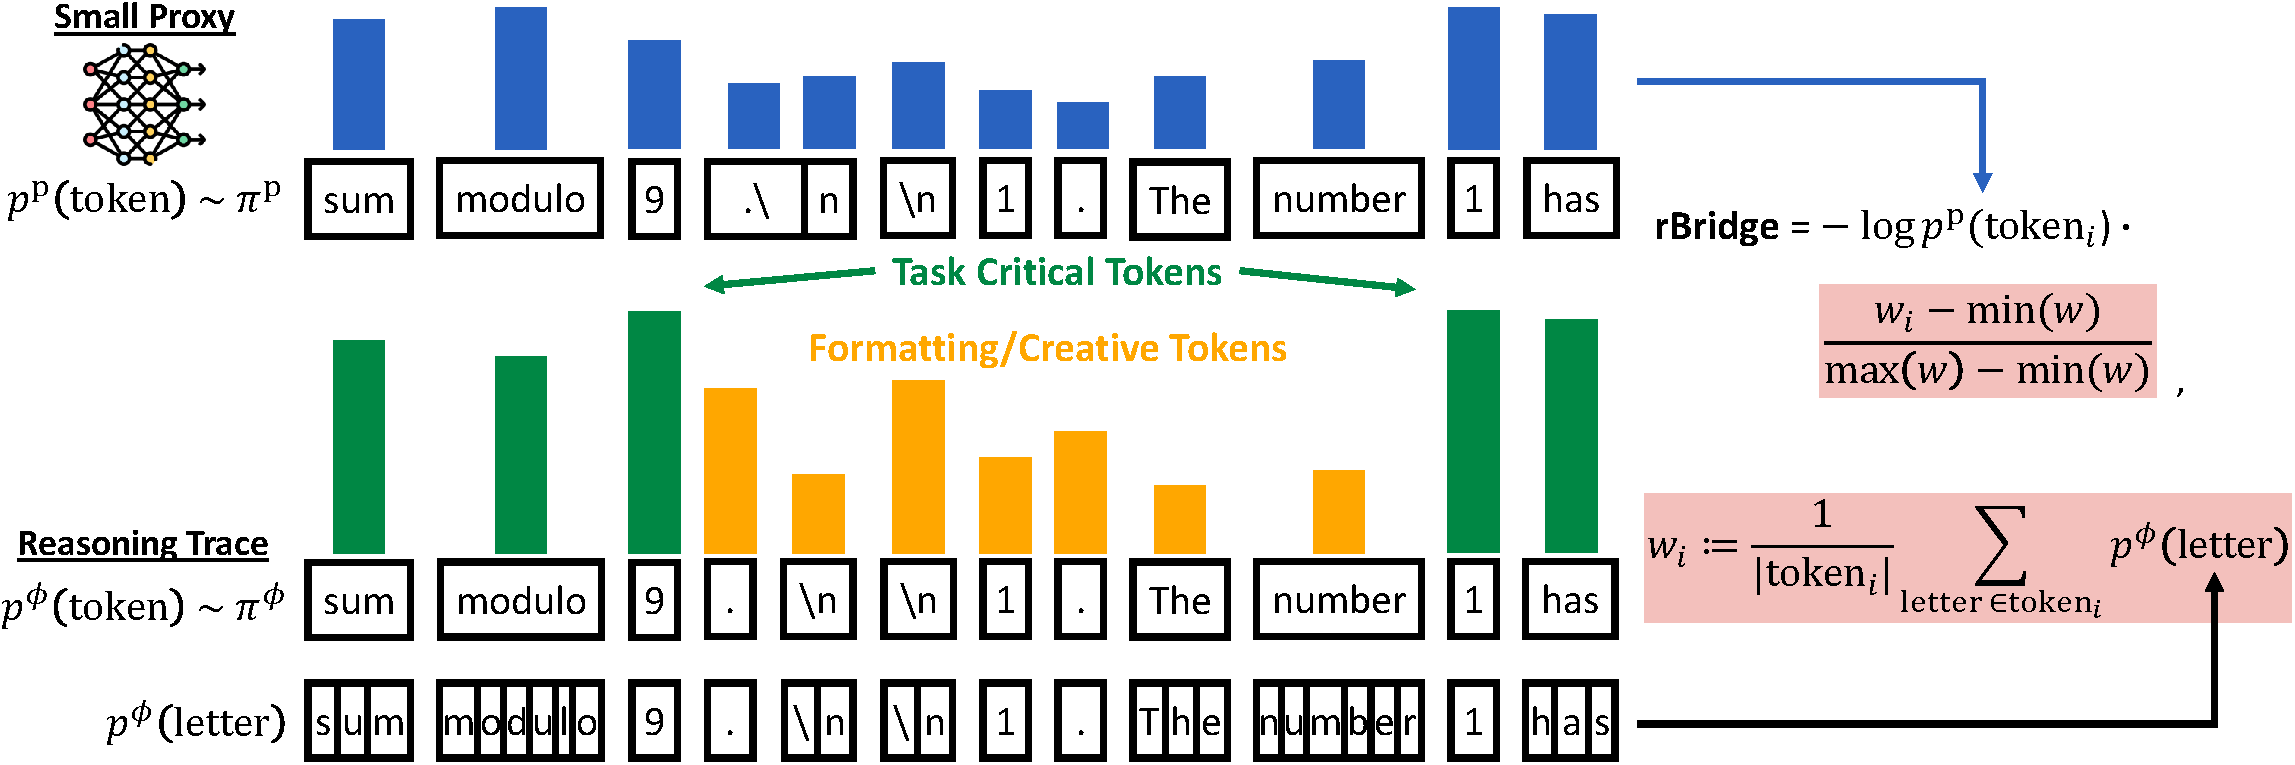
\includegraphics[width=\linewidth]{figs/rbridge3.pdf}
    \caption{Schematic overview of \tsc{rBridge}, which is used to predict and rank performance at much larger model size. We use a frontier model $\pi^\phi$'s reasoning trace \citep{NEURIPS2022_9d560961} as the gold label $Y^*$ and compute {\setlength{\fboxsep}{1pt}\colorbox{myred!30}{weighted}} NLL for evaluation. Each token $i$'s NLL is {\setlength{\fboxsep}{1pt}\colorbox{myred!30}{weighted}} by the frontier model's confidence in that token (MinMax normalized). To handle tokenizer mismatches between proxy and frontier models, we compute weights at the letter level and average within tokens.}
    \label{fig:rbridge}
\end{figure}

Pre-training modern language models at scale requires enormous computational and data resources, making it infeasible to exhaustively explore pre-training design choices directly at large scale \citep{radford2018improving, Radford2019, brown2020language, NEURIPS2019_c20bb2d9, hoffmann2022an,cottier2024rising,hu2024minicpm,khandelwal2024100,han2025trillion}. In response, leveraging smaller models as a proxy for larger model performance has been a key direction through the establishment of empirical scaling laws for prediction \citep{kaplan2020scaling,hoffmann2022training} or derivation of pre-training dataset rank invariance across scale \citep{magnusson2025datadecide}. 

However, the literature on the \textit{emergence} of reasoning performance as we scale model size \citep{wei2022emergent, almazrouei2023falcon, NEURIPS2024_5f1eee25} suggests that there may be a limit to how small theses proxy models can be. They demonstrate that reasoning capabilities only appear when models are sufficiently large in size. \citet{NEURIPS2024_5f1eee25}'s granular study demonstrates \textit{random} accuracy on small scale models of size 300M - 3B benchmarked on reasoning tasks like MMLU \citep{hendrycks2021measuring} and GSM8K \citep{cobbe2021training}. Contrarily, other non-reasoning benchmarks like TriviaQA \citep{joshi-etal-2017-triviaqa} and HellaSwag \citep{zellers-etal-2019-hellaswag} show smooth signs of improvement even at small scale. 

We further visualize this challenge of using small models to proxy large model especially for reasoning in Fig. \ref{fig:motivation}. While larger models exhibit stable Accuracy (Acc.) improvement (Fig. \ref{fig:13b32b}), smaller models are highly noisy, and in the case of the smallest 1B model, sloping in the wrong direction (Fig. \ref{fig:1b7b}).

%This challenge persists across mathematics, science, engineering, commonsense, and coding benchmarks visualized in in Appendix \ref{app:noisy}. \sungjun{Comment: unncessary I think.simply point to Appendix for details?}

Due to this limitation, practitioners are often constrained to relatively larger proxy models up to 15B to capture reasoning performance, which incurs substantial computational and economic costs \citep{grattafiori2024llama3herdmodels, deepseekai2025deepseekv3technicalreport}. For example, a single training run of a 7B model with 500B tokens can reportedly exceed 50K USD in cost \citep{han2025trillion}. 

% Alternatively, practitioners may resort to smaller models evaluated on smoothly scaling benchmarks \citep{liu2025regmix, xie2023doremi}, but they are suboptimal correlates of the target model's reasoning capabilities. 

\begin{figure}[tb]
    \centering
    \begin{subfigure}[b]{0.497\textwidth}
        \centering
        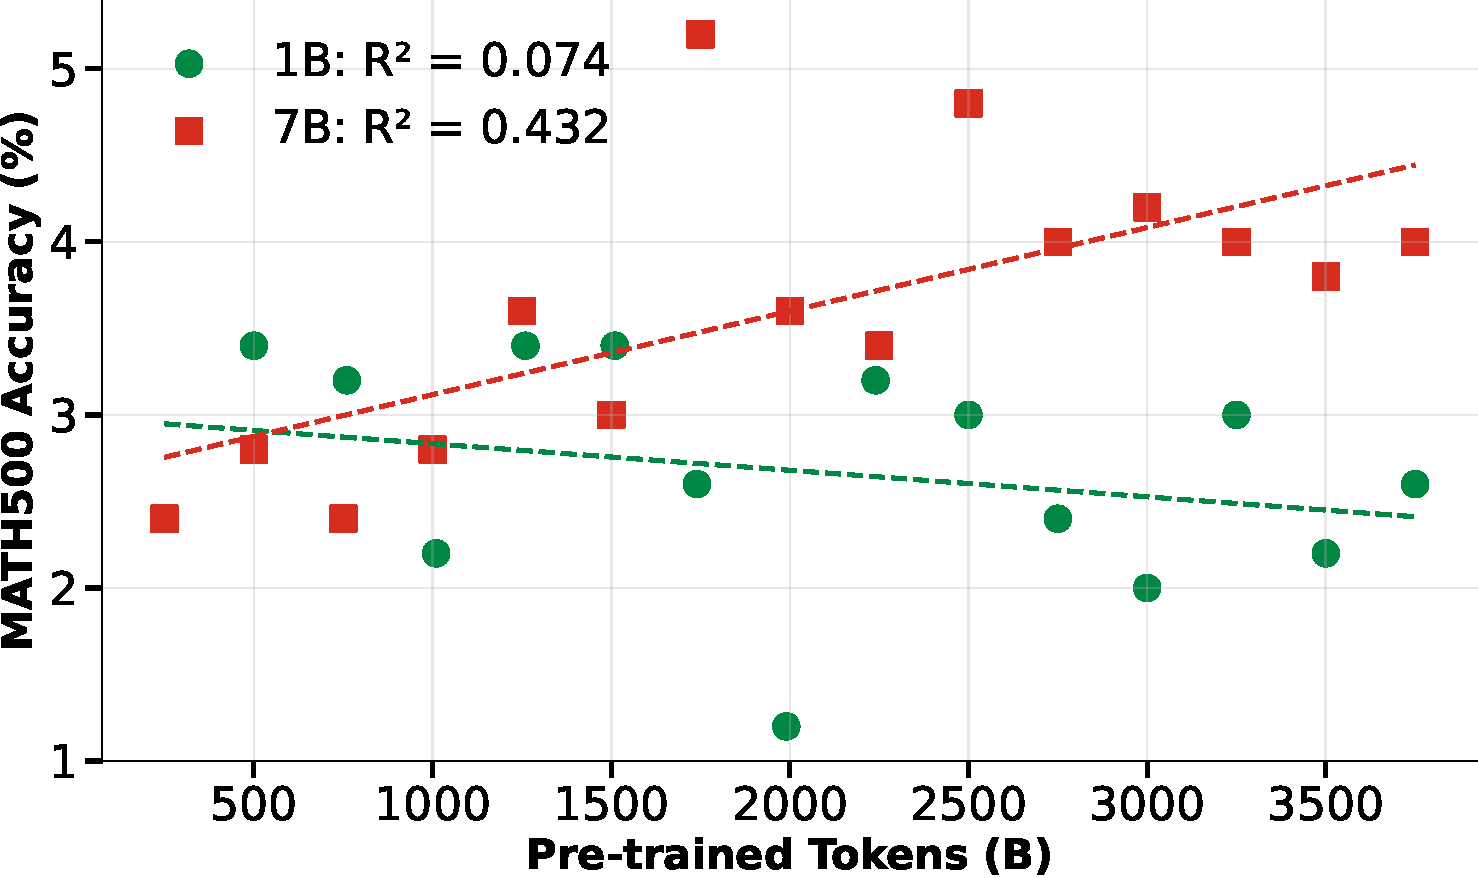
\includegraphics[width=\textwidth]{figs/math500_1b_7b_performance.pdf}
        \caption{Pre-training progress on 1B and 7B model}
        \label{fig:1b7b}
    \end{subfigure}
    \hfill
    \begin{subfigure}[b]{0.497\textwidth}
        \centering
        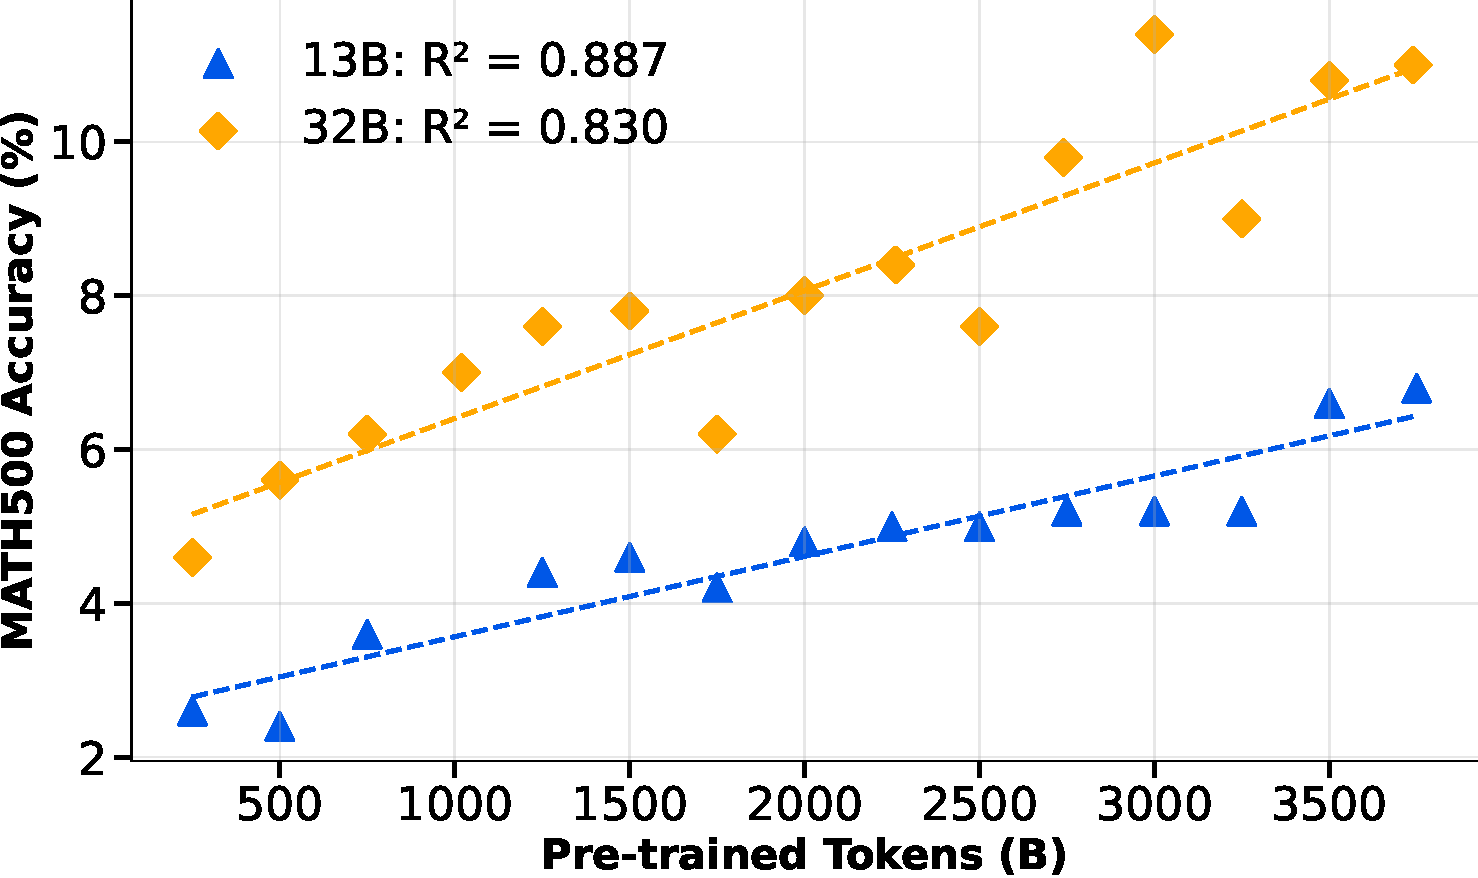
\includegraphics[width=\textwidth]{figs/math500_13b_32b_performance.pdf}
        \caption{Pre-training progress on 13B and 32B model}
        \label{fig:13b32b}
    \end{subfigure}
    \caption{Using MATH500 as an example benchmark, given the same data source OLMo-Mix-1124 \citep{olmo20242}, smaller models exhibit more noise and get the direction wrong, making it challenging to use smaller models to proxy larger model performance. R$^2$ values are derived from linear curve fitting. Extended visualization across other reasoning benchmarks are available in Appendix \ref{app:noisy}.}
    \label{fig:motivation}
\end{figure}

% To fill this literature gap, we raise the following research question: \textit{Can we effectively predict pre-trained large model's reasoning via small proxy model, and use these to rank datasets?}

% Our preliminary empirical studies analyzes indicate the limitation of standard negative log likelihood (NLL) and alternative innovations to the standard NLL.
 
\paragraph{Contribution.} To bridge the evaluation scheme at small proxy to large target scale, we first analyze limitations of past approaches (\textbf{\S\ \ref{sec:limit}}). Our analysis uncovers that existing methods fail to \textbf{(\S\ \ref{sec:limit} (1))} align with the pre-training objective, and \textbf{(\S\ \ref{sec:limit} (2))} align with the target task. \textbf{(1)} Alignment with the pre-training objective is required as small pre-trained models \textit{lack strong generalization capabilities}. \textbf{(2)} Ensuring that the evaluation scheme is aligned with the target task is necessary to fulfil our \textit{ultimate} goal of proxying task performance at large scale. To achieve \textbf{(1, 2)}, we use frontier-model generated gold reasoning traces \citep{NEURIPS2022_9d560961} for negative log-likelihood (NLL) (Fig. \ref{fig:rbridge}). Then, we further task alignment at the token-level by automatically weighting tokens based on their level of task-alignment (Fig. \ref{fig:rbridge}). We empirically validate our method \tsc{rBridge} (\textbf{\S\ \ref{sec:exp}}) in the following five ways:
\begin{enumerate}
    \item On a pre-training dataset ranking benchmark with target 1.2B scale, \tsc{rBridge} achieves \textbf{80.8\%} decision accuracy across \textbf{25} pre-training datasets, outperforming \textbf{5} baselines, reducing dataset ranking compute cost by at least \textbf{100.2$\times$} against the best .
    \item \tsc{rBridge} achieves best average proxy (1B) to target (13B, 32B) relationship across \textbf{6} benchmarks (mathematics, science, engineering, commonsense, and coding tasks), against \textbf{6} baselines. 
    \item \tsc{rBridge} achieves best average 1B $\rightarrow$ 13B relationship after a supervised fine-tuning (SFT) stage at target scale across \textbf{4} benchmarks, against \textbf{6} baselines.
    \item \tsc{rBridge} outperforms proxy models \textbf{7 - 13$\times$} larger using the target metric (e.g. Acc., Pass@K).
    \item Finally, we demonstrate that \tsc{rBridge}-target relationship on one pre-trained dataset can be \textbf{zero-shot transferred} to an alternative dataset for low-error performance prediction and ranking using a \textbf{fraction} of experimental compute cost.
\end{enumerate}

% Deprecated introduction

%For instance, \cite{xie2023doremi}, \cite{liu2025regmix} leverage proxy models (1 - 280M) to help optimize pre-training data mixture weights at target scale ($~$7B) operate under the notion that performance at very small scale have a meaningful relationship with larger scales \sungjun{Comment: I am afraid introducing this here might give the readers wrong idea that it is possible to optimize using very small proxy models targeting large models. My suggestion is to move this to a related work section where we can provide more details. I also mention the limitations of their method below in my text insert as well. }.

% A common strategy to mitigate this cost is to study proxy models: smaller models trained under constrained budgets to approximate how larger models might respond to different training conditions. These proxies enable systematic investigation of scaling behaviors while keeping experimentation tractable.

% Modern large language models' (LLMs) success can be largely attributed to the pre-training (self-supervised learning) and post-training paradigm \citep{radford2018improving, Radford2019, brown2020language, NEURIPS2019_c20bb2d9}. The large pre-training data size and corresponding model size allows for improved downstream performance and generalization \citep{groeneveld-etal-2024-olmo,isik2025scaling}. In this paradigm, pre-training notoriously consumes a significant amount of economic cost due to outsized compute costs \citep{hoffmann2022an,cottier2024rising,hu2024minicpm,khandelwal2024100,han2025trillion}. This high-cost problem is amplified as researchers search for optimal pre-training recipes \citep{NEURIPS2021_8df7c2e3}. 

% Therefore, it is unclear how reliable leveraging small proxy models ($\leq 1$B) to predict larger-scale target models is. \sungjun{Comment: with the above added context, we don't need this statement anymore - as we have strongly presented the case that <1B is just not reliable of larger target models}

% Past works utilize benchmarks that do not exhibit emergent behavior: \cite{xie2023doremi}, \cite{liu2025regmix}'s data mixture optimization study conducts experiments on non-emergent benchmarks like TriviaQA and HellaSwag \citep{NEURIPS2024_5f1eee25} \sungjun{Comment: Move this to a related work section.}.

% \begin{wrapfigure}{r}{0.4\textwidth} 
%   \vspace{-15pt}
%   \centering
%   \includegraphics[width=0.4\textwidth]{figs/diagram.pdf} 
%   \caption{High-level schematic diagram of evaluation scale transfer for pre-training.}\label{fig:diagram} 
%   \vspace{-5pt}
% \end{wrapfigure}

 % First, we empirically confirm that reasoning evaluation using the target metric (Accuracy or Pass@k) is highly noisy in smaller models (\textbf{\S\ \ref{sec:lack}}).
